\documentclass[11pt]{article}
\usepackage{iwslt15}
\usepackage{times}
\usepackage{url}
\usepackage{latexsym}
\usepackage{amsmath}
\usepackage{amssymb}
\usepackage{array}
\usepackage{algorithm}
\usepackage[noend]{algpseudocode}
\usepackage{booktabs}
\usepackage{tikz}
\usepackage{forest}
\usepackage{subcaption}

\usepackage{tikz}
\usepackage{pgfplots}
\usepackage{enumitem}
\setlist{noitemsep}

\pgfplotsset{compat=newest}
\usepgfplotslibrary{groupplots}

\pgfplotsset{try min ticks=6}

\definecolor{bblue}{HTML}{4F81BD}
\definecolor{rred}{HTML}{C0504D}
\definecolor{ggreen}{HTML}{9BBB59}
\definecolor{ppurple}{HTML}{9F4C7C}
\definecolor{oorange}{HTML}{F08000}
  
\emergencystretch 3em


\title{Is Neural Machine Translation Ready for Deployment? \\ A Case Study on 30 Translation Directions}

\author{Marcin Junczys-Dowmunt\textsuperscript{1,2}, Tomasz Dwojak\textsuperscript{1,2}, Hieu Hoang\textsuperscript{3} \\
\textsuperscript{1}Faculty of Mathematics and Computer Science, Adam Mickiewicz University in Pozna\'{n}\\
\textsuperscript{2}School of Informatics, University of Edinburgh \\
\textsuperscript{3}Moses Machine Translation CIC\\
{\tt \normalsize junczys@amu.edu\pgfplotsset{try min ticks=3}.pl t.dwojak@amu.edu.pl}\\
{\tt \normalsize hieu@hoang.co.uk }}

\date{}

\begin{document}
 \maketitle
\begin{abstract}
In this paper we provide the largest published comparison of translation quality for phrase-based SMT and neural machine translation across 30 translation directions. For ten directions we also include hierarchical phrase-based MT. Experiments are performed for the recently published United Nations Parallel Corpus v1.0 and its large six-way sentence-aligned subcorpus. 
In the second part of the paper we investigate aspects of translation speed, introducing AmuNMT, our efficient neural machine translation decoder. We demonstrate that current neural machine translation could already be used for in-production systems when comparing words-per-second ratios.

\end{abstract}

\section{Introduction}

We compare the performance of phrase-based SMT, hierarchical phrase-based, and neural machine translation (NMT) across fifteen language pairs and thirty translation directions. \cite{ZIEMSKI16.1195} recently published the United Nations Parallel Corpus v1.0. It contains a subcorpus of ca.~11M sentences fully aligned across six languages (Arabic, Chinese, English, French, Russian, and Spanish) and official development and test sets, which makes this an ideal resource for experiments across multiple language pairs. It is also a compelling use case for in-domain translation with large bilingual in-house resources. We provide BLEU scores for the entire translation matrix for all official languages from the fully aligned subcorpus. 

We also introduce AmuNMT\footnote{\url{https://github.com/emjotde/amunmt}}, our efficient neural machine translation decoder and demonstrate that the current set-up could already be used instead of Moses in terms of translation speed when a single GPU per machine is available. Multiple GPUs would surpass the speed of the proposed in-production Moses configuration by far. 

\section{Training data}

\subsection{The UN corpus}

The United Nations Parallel Corpus v1.0 \cite{ZIEMSKI16.1195} consists of human translated UN documents from the last 25 years (1990 to 2014) for the six official UN languages, Arabic, Chinese, English, French, Russian, and Spanish. Apart from the pairwise aligned documents, a fully aligned subcorpus for the six official UN languages is distributed. This subcorpus consists of sentences that are consistently aligned across all languages with the English primary documents. Statistics for the data are provided below:

\begin{table}[h]
\centering \setlength{\arrayrulewidth}{1pt}
\begin{tabular}{|c|c|c|}
\hline
Documents & Lines & English Tokens \\ \hline
86,307 & 11,365,709 & 334,953,817 \\ \hline
\end{tabular} 
\caption{Statistics for fully aligned subcorpus}
\label{tab.statistics.fully}
\end{table}

Documents released in 2015 (excluded from the main corpus) were used to create official development and test sets for machine translation tasks. Development data was randomly selected from documents that were released in the first quarter of 2015 and test data was selected from the second quarter. 
Both sets comprise 4,000 sentences that are 1-1 alignments across all official languages. As in the case of the fully aligned subcorpus, any translation direction can be evaluated.

\subsection{Preprocessing}

Sentences longer than 100 words were discarded. We lowercased the training data as it was done in \cite{ZIEMSKI16.1195}; the data was tokenized with the Moses tokenizer. For Chinese segmentation we used Jieba\footnote{\url{https://github.com/fxsjy/jieba}} before applying the Moses tokenizer. 

\subsection{Subword units}

To avoid the large-vocabulary problem in NMT models \cite{44929}, we use byte-pair-encoding (BPE) to achieve open-vocabulary translation with a fixed vocabulary of subword symbols \cite{DBLP:journals/corr/SennrichHB15}. For all languages we set the number of subword units to 30,000. Segmentation into subword units is applied after any other preprocessing step. During evaluation, subwords are concatenated to form full tokens. 

\section{Phrase-based SMT baselines}
\label{pbmtbaselines}
In \cite{ZIEMSKI16.1195}, we provided baseline BLEU scores for Moses \cite{Koehn:2007:MOS:1557769.1557821} configurations that were trained on the 6-way subcorpus. We repeat the system description here:

To speed up the word alignment procedure, we split the training corpora into four equally sized parts that are aligned with MGIZA++ \cite{Gao:2008:PIW:1622110.1622119}, running 5 iterations of Model 1 and the HMM model on each part.\footnote{We confirmed that there seemed to be no quality loss due to splitting and limiting the iterations to simpler alignment models.}
We use a 5-gram language model trained from the target parallel data, with 3-grams or higher order being pruned if they occur only once. Apart from the default configuration with a lexical reordering model, we add a 5-gram operation sequence model \cite{conf/acl/DurraniFSHK13} (all n-grams pruned if they occur only once) and a 9-gram word-class language model with word-classes produced by word2vec \cite{journals/corr/abs-1301-3781} (3-grams and 4-grams are pruned if they occur only once, 5-grams and 6-grams if they occur only twice, etc.), both trained using KenLM \cite{Heafield-estimate}.  To reduce the phrase-table size, we apply significance pruning \cite{Johnson07improvingtranslation} and use the compact phrase-table and reordering data structures \cite{junczys_mtm_2012}.
During decoding, we use the cube-pruning algorithm with stack size and cube-pruning pop limits of 1,000. This configuration is the actual setting used at the United Nations for their in-house translation system.

\begin{figure*}[p]
\centering
\begin{tikzpicture}

\begin{groupplot}[group style={group size=1 by 3},ymajorgrids,
ybar=0pt,
 ymin=0,
 width=\textwidth,
 height=0.33\textheight,
 ymin=21, ymax=69,
 xtick=data,% crucial line for the xticklabels directive
 nodes near coords={\pgfmathprintnumber[fixed zerofill, precision=1]{\pgfplotspointmeta}},
 every node near coord/.append style={
  white,  
  rotate=90, anchor=west, xshift=-10.5mm, font=\boldmath
 },
 xticklabels from table={compare.dat}{lp},
 xticklabel style={text height=2ex}]

\nextgroupplot[xmin=0.5,xmax=10.5,bar width=15pt,legend style={cells={anchor=west}}]
\addplot[bblue,fill=bblue,mark=none] table[y=pb,x=xpos]{compare.dat};
\addplot[rred,fill=rred,mark=none] table[y=nmt4,x=xpos]{compare.dat};
\legend{\strut\; Pb-SMT, \strut\; NMT 1.2M}

\nextgroupplot[xmin=10.5,xmax=20.5,bar width=15pt]
\addplot[bblue,fill=bblue,mark=none] table[y=pb,x=xpos]{compare.dat};
\addplot[rred,fill=rred,mark=none] table[y=nmt4,x=xpos]{compare.dat};

\nextgroupplot[xmin=20.5,xmax=30.5,bar width=15pt]
\addplot[bblue,fill=bblue,mark=none] table[y=pb,x=xpos]{compare.dat};
\addplot[rred,fill=rred,mark=none] table[y=nmt4,x=xpos]{compare.dat};

\end{groupplot}
\end{tikzpicture}
\caption{Comparison between Moses baseline systems and neural models for the full language pair matrix of the 6-way corpus.}\label{pbsmtnmt1}
\end{figure*}

\section{Neural translation systems}

The neural machine translation system is an attentional encoder-decoder \cite{DBLP:journals/corr/BahdanauCB14}, which has been trained with Nematus  \cite{DBLP:conf/wmt/SennrichHB16}.
We used mini-batches of size 40, a maximum sentence length of 100, word embeddings of size 500, and hidden layers of size 1024.
We clip the gradient norm to 1.0 \cite{DBLP:conf/icml/PascanuMB13}.
Models were trained with Adadelta \cite{DBLP:journals/corr/abs-1212-5701}, reshuffling the training corpus between epochs.
The models have been trained model for 1.2M iterations (one iteration corresponds to one mini-batch), saving every $30,000$ iterations. On our NVidia GTX 1080 this corresponds to roughly 4 epochs and 8 days of training time. Models with English as there source or target data were trained for another 1.2M iterations (another 2 epochs, 8 days) to test the influence of increased training time. For ensembling/averaging, we chose the last four model checkpoints.

\section{Phrase-based vs. NMT -- full matrix}
In Figure~\ref{pbsmtnmt1} we present the results for all thirty language pairs in the United Nations parallel corpus for the officially included test set. Here we compare with NMT models that were trained for 4 epochs or 1.2M iterations. With the exception of fr-es and ru-en the neural system is always comparable or better than the phrase-based system. The differences where NMT is worse are very small. Especially in cases where Chinese is one of the languages in a language pair, the improvement of NMT over PB-SMT is dramatic with between 7 and 9 BLEU points. 
We also see large improvements for translations out of and into Arabic. It should be noted here, that no special preprocessing has been applied for Arabic. It is interesting to observe that improvements are present also in the case of the highest scoring translation directions, en-es and es-en.

\section{Phrase-based vs. Hiero vs. NMT -- language pairs with English}

\begin{figure*}[t]
\centering
\begin{tikzpicture}
\begin{groupplot}[group style={group size=1 by 2},ymajorgrids,
ybar=0pt,
 ymin=0,
 width=\textwidth,
 height=0.33\textheight,
 ymin=31, ymax=69,
nodes near coords={\pgfmathprintnumber[fixed zerofill, precision=1]{\pgfplotspointmeta}},
 every node near coord/.append style={
  white, 
  rotate=90, anchor=west, xshift=-10.5mm, font=\boldmath
 },
 xtick=data,% crucial line for the xticklabels directive
 xticklabels from table={hiero.dat}{lp},
 xticklabel style={text height=2ex}]

\nextgroupplot[xmin=0.5,xmax=5.5,bar width=15pt,legend style={cells={anchor=west}}]
\addplot[bblue,fill=bblue,mark=none] table[y=pb,x=xpos]{hiero.dat};
\addplot[ppurple,fill=ppurple,mark=none] table[y=hiero,x=xpos]{hiero.dat};
\addplot[rred,fill=rred,mark=none] table[y=nmt4,x=xpos]{hiero.dat};
\addplot[oorange,fill=oorange,mark=none] table[y=2nmt4,x=xpos]{hiero.dat};
\legend{\strut\; Pb-SMT, \strut\; Hiero, \strut\; NMT 1.2M, \strut\; NMT 2.4M}

\nextgroupplot[xmin=5.5,xmax=10.5,bar width=15pt]
\addplot[bblue,fill=bblue,mark=none] table[y=pb,x=xpos]{hiero.dat};
\addplot[ppurple,fill=ppurple,mark=none] table[y=hiero,x=xpos]{hiero.dat};
\addplot[rred,fill=rred,mark=none] table[y=nmt4,x=xpos]{hiero.dat};
\addplot[oorange,fill=oorange,mark=none] table[y=2nmt4,x=xpos]{hiero.dat};

\end{groupplot}
\end{tikzpicture}
\caption{For all language pairs involving English, we experimented also with hierarchal machine translation and more training iterations for the neural models. NMT 1.2M means 1.2 million iterations with a batch size of 40, training time ca. 8 days. NMT 2.4 means 2.4 million iterations accordingly.}\label{pbsmtnmt2}
\end{figure*}

The particularly impressive results for any translation direction involving Chinese motived us to experiment with hierarchical phrase-based machine translation (Hiero) as well. Hiero has been confirmed to outperform phrase-based SMT for the Chinese-English language pair. We further decided to expand our experiment with all language pairs that include English, as these are the main translation directions the United Nations are working with. For these ten translation directions we created a hierarchical PB-SMT system with the same preprocessing settings as the PB-SMT system. We also continued training of our neural systems for another four epochs or 1.2M iterations (2.4M in total) which increased training time to 16 days in total per neural system. 


\begin{figure*}[t]
\centering
\begin{subfigure}[t]{0.43\textwidth}
 \begin{tikzpicture}
\begin{axis}[
enlargelimits=0.1,
width=\textwidth,
height=0.35\textheight,
xlabel=Beam size,
ytick pos=left,
ymin=50, ymax=600,
xmin=1, xmax=20,
ylabel=Words per second (Wps)]
\addplot[bblue,mark=o,thick] plot coordinates {
( 1, 561.5) %18.9 - 17
( 2, 494.8)
( 3, 445.9)
( 4, 438.1)
( 5, 409.4)
( 6, 347.2)
( 7, 319.7)
( 8, 296.3)
(10, 280.2)
(12, 275.1)
(15, 244.4)
(20, 239.0)
};\label{words}
\end{axis}
\begin{axis}[
legend style={at={(0.95,0.5)},anchor=east},
y tick label style={
        /pgf/number format/.cd,
            fixed,
            fixed zerofill,
            precision=1,
        /tikz/.cd
    },
enlargelimits=0.1,
width=\textwidth,
height=0.35\textheight,
ymin=48, ymax=50,
xmin=1, xmax=20,
axis y line*=right]
\addlegendimage{/pgfplots/refstyle=words}\addlegendentry{Wps}
\addplot[rred,mark=*,thick] plot coordinates {
( 1, 47.99)
( 2, 49.27)
( 3, 49.52) 
( 4, 49.59)
( 5, 49.68)
( 6, 49.75)
( 7, 49.78)
( 8, 49.83)
(10, 49.77)
(12, 49.78)
(15, 49.83)
(20, 49.85)
}; \addlegendentry{Bleu}
\end{axis}
\end{tikzpicture}
\end{subfigure}\hspace{10mm}%
\begin{subfigure}[t]{0.43\textwidth}
 \begin{tikzpicture}
\begin{axis}[
enlargelimits=0.1,
width=\textwidth,
height=0.35\textheight,
xlabel=Beam size,
ytick pos=left,
ymin=50, ymax=600]
\addplot[bblue,mark=o,thick] plot coordinates {
(20, 239.0)
(30, 210.5)
(40, 197.8)
(50, 176.4)
(70, 140.7)
(100, 113.3)
(200, 63.5)
};\label{words}
\end{axis}
\begin{axis}[
legend style={at={(0.95,0.5)},anchor=east},
y tick label style={
        /pgf/number format/.cd,
            fixed,
            fixed zerofill,
            precision=1,
        /tikz/.cd
    },
enlargelimits=0.1,
width=\textwidth,
ymin=48, ymax=50,
height=0.35\textheight,
axis y line*=right,ylabel=Bleu]
\addlegendimage{/pgfplots/refstyle=words}\addlegendentry{Wps}
\addplot[rred,mark=*,thick] plot coordinates {
(20, 49.85)
(30, 49.85)
(40, 49.86)
(50, 49.90)
(70, 49.90)
(100, 49.89)
(200, 49.90)
}; \addlegendentry{Bleu}
\end{axis}
\end{tikzpicture}
\end{subfigure}
\caption{Beam size versus speed and quality for a single English-French model. Speed was evaluated with AmuNMT on a single GPU.}\label{beam}
\end{figure*}

Figure \ref{pbsmtnmt2} summarizes the results. As expected, Hiero outperforms PB-SMT by a significant margin for Chinese-English and English-Chinese, but does not even reach half the improvement of the NMT systems. For the other languages pairs we see mixed results; for French-English and Russian-English, where results for PB-SMT and NMT were very close, Hiero is actually the best system (TODO: Missing results here for the 2.4M iterations).

Training the NMT system for another eight days always improves the performance of the NMT system, but gains are rather small between 0.4 and 0.7 BLEU. We did not observe any improvements beyond 2M iterations. For our setting, it seems that stopping training after 8-10 days is a viable heuristic with little loss in terms of BLEU. Training with other corpus sizes, architectures, and sets of hyperparameters may behave differently.

To summarize the first part of this work: choosing NMT over PB-SMT seem like a good bet with results that reach from comparable to far superior in terms of BLEU. In the future we would like to verify these results with  human evaluation.

\section{Efficient decoding with AmuNMT}
AmuNMT\footnote{\url{http://github.com/emjotde/amunmt}} is a ground-up neural MT toolkit implementation, developed in C++. It currently consist of an efficient beam-search inference engine for models trained with Nematus. We focused mainly on efficiency and usability. Features of the AmuNMT decoder include:

\begin{itemize}
 \item Low-latency CPU-based decoding with intra-sentence multi-threading (one sentence makes use of multiple threads during matrix operations) and sentence-wise threads (different sentences are decoded in different threads);
 \item Multi-GPU support for sentence-wise translation per GPU;
 \item Full compatibility with NMT models trained with Nematus \cite{DBLP:conf/wmt/SennrichHB16};
 \item Ensembling of similar models;
 \item Ensembling of models with the same output vocabulary but different inputs. A similar configuration was used in the winning system for the automatic post-editing shared task at WMT2016 \cite{DBLP:journals/corr/Junczys-Dowmunt16}.
 \item YAML vocabularies and configuration files; % TODO is this a big deal?
 \item Integrated segmentation into subword units and de-segmentation \cite{DBLP:journals/corr/SennrichHB15};
 \item A clean and documented C++ code-base.
\end{itemize}


\begin{figure*}[t]
\centering
\begin{subfigure}[t]{0.35\textwidth}
\begin{tikzpicture}
\begin{axis}[
    ybar,
    width=\textwidth,
    ymajorgrids,
    height=0.35\textheight,
	bar width=15pt,
    enlargelimits=0.15,
    ylabel={Words per second},
    xtick={1 ,2 ,3 },
    xticklabels={Google CPU x88,
Google GPU T-K80,
Google TPU},
    xmin=0.75, xmax=3.25,
    ymin=50, ymax=1200,
    x tick label style={rotate=45,anchor=east, yshift=-0.2cm},
    ]
\addplot+[ybar, ppurple, nodes near coords, text=black] plot coordinates {
(1, 104.2)
(2, 45.5)
(3, 358.8)
};
\end{axis}
\end{tikzpicture}
\caption{Words per second for Google NMT system reported by \cite{google}. We only give this as an example for a production-ready system.}\label{speedgoogle}
\end{subfigure}\hspace{4mm}
\begin{subfigure}[t]{0.6\textwidth}
\begin{tikzpicture}
\begin{axis}[
    ybar,
    width=\textwidth,
    ymajorgrids,
    height=0.35\textheight,
	bar width=15pt,
    enlargelimits=0.15,
    %ylabel={Words per second},
    xtick={1 ,2 ,3, 4 ,5, 6},
    xticklabels={
    Moses CPU x16,
    Nematus CPU x16,
    Nematus GPU x1,
    AmuNMT CPU x16,
    AmuNMT GPU x1,
    AmuNMT GPU x4
    },
    xmin=0.75, xmax=6.25,
    ymin=50, ymax=1200,
    x tick label style={rotate=45,anchor=east, yshift=-0.2cm},
    ]
\addplot+[ybar, oorange, nodes near coords, text=black] plot coordinates {
% 118553
(1, 455.3)
(2, 47.4)
(3, 269.4)
(4, 116.8) % 1248.7
(5, 409.4) % 431
(6, 1202.3) % 118.5 
};

\end{axis}
\end{tikzpicture}
\caption{Moses vs. Nematus vs.~AmuNMT: Our CPUs are Intel Xeon E5-2620 2.40GHz, our GPUs are GeForce GTX 1080. CPU x16 means 16 CPU threads, GPU x1 means single GPU, GPU x4 means multi-GPU mode. All NMT systems were run with a beam size of 5.}\label{speedamun}
\end{subfigure}
\caption{Comparison of translation speed in words per second}\label{speed1}
\end{figure*}



\subsection{Beam size vs. Speed and Quality}

Beam size has a large impact on decoding speed. In Figure~\ref{beam} we plot the influence of beam size on decoding speed (as words per second) and translation quality (in BLEU) for the English-French model. The English part of the UN test set consists or ca. 120.000 tokens, the whole test sets was translated for each experiment. As can be seen, beam sizes beyond 5-7 do not result in significant improvements as the quality for a beam size of 5 is only 0.1 BLEU below the maximum. However, decoding speed is significantly slower. We therefore choose a beam-size of 5 for our experiments.  

%\subsection{Checkpoint ensembling vs. averaging}

\subsection{AmunNMT vs. Moses and Nematus}

In Figure~\ref{speedgoogle} we report speed in terms of words per second as provided by \cite{google}. Although the models of \cite{google} are more complex that our own, we treat the reported figures as a reference of deployment-ready performance for NMT. 

We ran our experiments on an Intel Xeon E5-2620 2.40GHz server with four NVIDIA GeForce GTX 1080 GPUs. The phrase-based parameters are described in Section~\ref{pbmtbaselines} which is guided by best practises to achieving reasonable speed vs. quality trade-off \cite{junczys_mtsummit_2013}. The neural MT models are as described in the previous section.

We present the words-per-second ratio for our NMT models using AmunNMT and Nematus, executed on the CPU and GPU, Figure~\ref{speedamun}. For the CPU version we use 16 threads, translating one sentence per thread. We restrict the number of OpenBLAS threads to 1 per main Nematus thread, restricting the total number of threads to 16. For the GPU version of Nematus we use 5 processes to maximize GPU saturation. As a baseline, the phrase-based model reaches 455 words per second using 16 threads.

The CPU-bound execution of Nematus reaches 47 words per second while the GPU-bound achieved 270 words per second. 

In similar settings, the CPU-bound AmuNMT is 2.5 times faster than Nematus, but still nearly four times slower than Moses. However, the GPU-executed version 1.5 time faster than Nematus and is almost as fast as Moses, achieving 409 words per second. The similar translation speed will allow us to replace a Moses-based SMT system with an AmunNMT-based NMT system in a production environment without severely affecting translation throughput. 

AmuNMT can parallelize to multiple GPUs present in one machine by processing one sentence per GPU. Translation speed increases almost linearly to 1,200 words per second with four GPUs. 
AmuNMT has a start-up time of less than 10 seconds, while Nematus may need several minutes until the first translation can be produced. Nevertheless, the model used in AmuNMT is an exact implementation of the Nematus model that produces identical results.

The size of the NMT model with the chosen parameters is approximately 300 MB, which means about 24 models could be loaded onto a single GPU with 8GB of RAM. Hardly any overhead is required during translation. With multiple GPUs, access could be parallelized and optimally scheduled in a query-based server setting. 

\subsection{Low-latency translation}

\begin{figure}[t]
\centering
\begin{tikzpicture}
\begin{axis}[
    ybar,
    width=0.48\textwidth,
    ymajorgrids,
    height=0.28\textheight,
	bar width=15pt,
   enlargelimits=0.15,
    ylabel={Latency -- seconds per sentence},
    xtick={1 ,2 ,3, 4 ,5},
    xticklabels={
    Moses CPU,
    Nematus CPU,
    Nematus GPU,
    AmuNMT CPU,
    AmuNMT GPU,
    },
    %xmin=0.75, xmax=5.25,
    x tick label style={rotate=45,anchor=east, yshift=-0.2cm},
    y tick label style={
        /pgf/number format/.cd,
            fixed,
            fixed zerofill,
            precision=1,
        /tikz/.cd
    },
    ]
\addplot+[ybar, oorange, nodes near coords, text=black] plot coordinates {
(1, 0.71)
(2, 8.54)
(3, 0.61)
(4, 2.88)
(5, 0.14)
};

\end{axis}
\end{tikzpicture}
\caption{Translation latency measured in seconds per sentence, NMT systems were run with a beam size of 5. Translations were executed serially.}\label{latency}
\end{figure}

Until now, we have evaluated translation speed as the time it takes to translate a large test set using a large number of cores on a powerful server. This bulk-throughput measure is useful for judging the performance of the MT system for batch translation of large number of documents.
 
However, there are use-cases where the latency for a single sentence may be important, for example, interactive or predictive translation \cite{Knowles}. %Other settings will be located between these extremes --- low-latency translation and bulk-translation --- as for example MT usage in CAT systems, another instance of interactive translation. 
To compare per-sentence latency we translate our test set with all tools in a serial fashion, using at most one CPU thread or process. We do not aim at full GPU saturation as this would not improve latency. We then average time over the number of sentences and report seconds per sentence in Figure~\ref{latency}, lower values are better. Here AmuNMT GPU compares very favourably against all other solutions with a 5 times smaller latency than Moses and a more than 4 times smaller latency that Nematus. Latency between the CPU-only variants shows the same ratios as bulk-translation in the previous section. %(TODO: evaluate latency with multiple CPU-threads per sentence.)

\section{Conclusions}

We evaluated the performance of neural machine translation on all thirty translation directions of the United Nations Parallel Corpus v1.0. We showed that for nearly all translation directions NMT is either on par with or surpasses phrase-based SMT. There seems to be no risk in potential quality loss due to switching to NMT. For some language pairs, the gains are substantial, as measured by BLEU. These include all pairs that have Chinese as a source or target language. Very respectable gains can also be observed for Arabic. For other language pairs there is generally at least some improvement. 

Although NMT systems are known to generalize better than phrase-based systems for out-of-domain data, it was unclear how they perform in a purely in-domain setting which is of interest for any larger organization with significant resources of their own data, such as the UN or other governmental bodies. This work currently lacks human evaluation which we would like to supply in future versions. 

We introduced our efficient neural machine translation beam-search decoder, AmuNMT, and demonstrated that high-quality and high-performance neural machine translation can be achieved on commodity hardware; the GPUs we tested on are widely available to the general public for gaming PCs and graphics workstations. A single GPU matches the performance of 16 CPU threads on server-grade Intel Xeon CPUs. We can take advantage of multiple GPUs to increase translation speed even further. Access to specialized hardware like Google's Tensor Processing Units seems unnecessary when planning to switch to neural machine translation using lower-parametrized models. 

Even the performance of the CPU-only version of AmuNMT allows to set-up demo systems and can be a viable solution for low-throughput settings. Training, however, requires a GPU. Still, one might start with one GPU for training and reuse the CPU machines on which Moses has been running  for first deployment. For future work, we plan to further improve the performance of AmuNMT, especially for CPU-only settings.

%\section{Acknowledgments}
%This project has received funding from the European Union's Horizon 2020 research and innovation
%programme under grant agreement 688139 (SUMMA).


\bibliography{un}
\bibliographystyle{IEEEtran}


\end{document}
